\section{آموزش مدل تشخیص چهره با \lr{YOLO}}

در این بخش از تمرین، هدف آماده‌سازی پایگاه داده \lr{WIDER FACE} و استفاده از یادگیری انتقالی (\lr{Transfer Learning}) برای آموزش مدل سبک \lr{YOLOv8n} جهت تشخیص چهره است. با توجه به اینکه کدهای کامل در فایل نوت‌بوک (\lr{Jupyter Notebook}) پیوست شده است، در این گزارش صرفاً به بررسی بخش‌های کلیدی پیاده‌سازی و تحلیل نتایج می‌پردازیم.

\subsection{منطق تبدیل مختصات دادگان}

پایگاه داده \lr{WIDER FACE} مختصات چهره‌ها را به صورت مختصات مطلقِ گوشه‌ی بالا-چپ و ابعاد \lr{(x, y, w, h)} ارائه می‌دهد. شبکه‌های خانواده \lr{YOLO} برای آموزش به مختصات نرمالایز شده‌ی مرکزِ شیء و ابعاد آن نیاز دارند.

\begin{codebox}[\lr{Core Normalization Logic}]
\begin{lstlisting}[language=Python]
# x, y, w, h: Absolute coordinates from WIDER FACE
# w_img, h_img: Image dimensions

x_center = (x + w / 2.0) / w_img
y_center = (y + h / 2.0) / h_img
w_norm = w / w_img
h_norm = h / h_img

# Class ID for face is set to 0
out_f.write(f"0 {x_center:.6f} {y_center:.6f} {w_norm:.6f} {h_norm:.6f}\n")
\end{lstlisting}
\end{codebox}

\begin{notebox}[اهمیت نرمال‌سازی]
دلیل تقسیم کردن مختصات بر ابعاد تصویر (\lr{w\_img} و \lr{h\_img}) این است که مدل نسبت به رزولوشن ورودی مستقل (\lr{Scale-Invariant}) شود. با این کار، تمام مقادیر در بازه $[0, 1]$ قرار می‌گیرند و همگرایی مدل در طول آموزش با سرعت و ثبات بیشتری انجام می‌شود.
\end{notebox}

\subsection{پیکربندی و تنظیمات آموزش}

پس از آماده‌سازی برچسب‌ها، فایل تنظیمات \lr{YAML} ساخته شده و مدل پایه‌ی \lr{YOLOv8n} (نسخه‌ی نانو) برای آموزش فراخوانی می‌شود.

\begin{codebox}[\lr{Training Configuration}]
\begin{lstlisting}[language=Python]
data_config = {
    'path': '/content',
    'train': 'WIDER_train/images',
    'val': 'WIDER_val/images',
    'nc': 1,
    'names': {0: 'face'}
}
# Save to face_data.yaml and start training
model = YOLO("yolov8n.pt")
results = model.train(data="face_data.yaml", epochs=10, imgsz=640)
\end{lstlisting}
\end{codebox}

\begin{tipbox}[انتخاب هایپرپارامترها]
در این آزمایش، به دلیل محدودیت منابع و زمان، تعداد \lr{Epoch}ها روی عدد ۱۰ تنظیم شد. همچنین سایز تصویر ورودی (\lr{imgsz=640}) انتخاب گردید تا تعادل مناسبی بین سرعت پردازش و دقت تشخیصِ چهره‌های کوچک برقرار شود.
\end{tipbox}

\subsection{تحلیل نمودارها و متریک‌های یادگیری}

پس از پایان ۱۰ دور آموزش، متریک‌های ارزیابی شبکه استخراج شدند. بررسی این نمودارها اطلاعات دقیقی از رفتار مدل در طول بهینه‌سازی به ما می‌دهد.

\begin{figure}[h!]
    \centering
    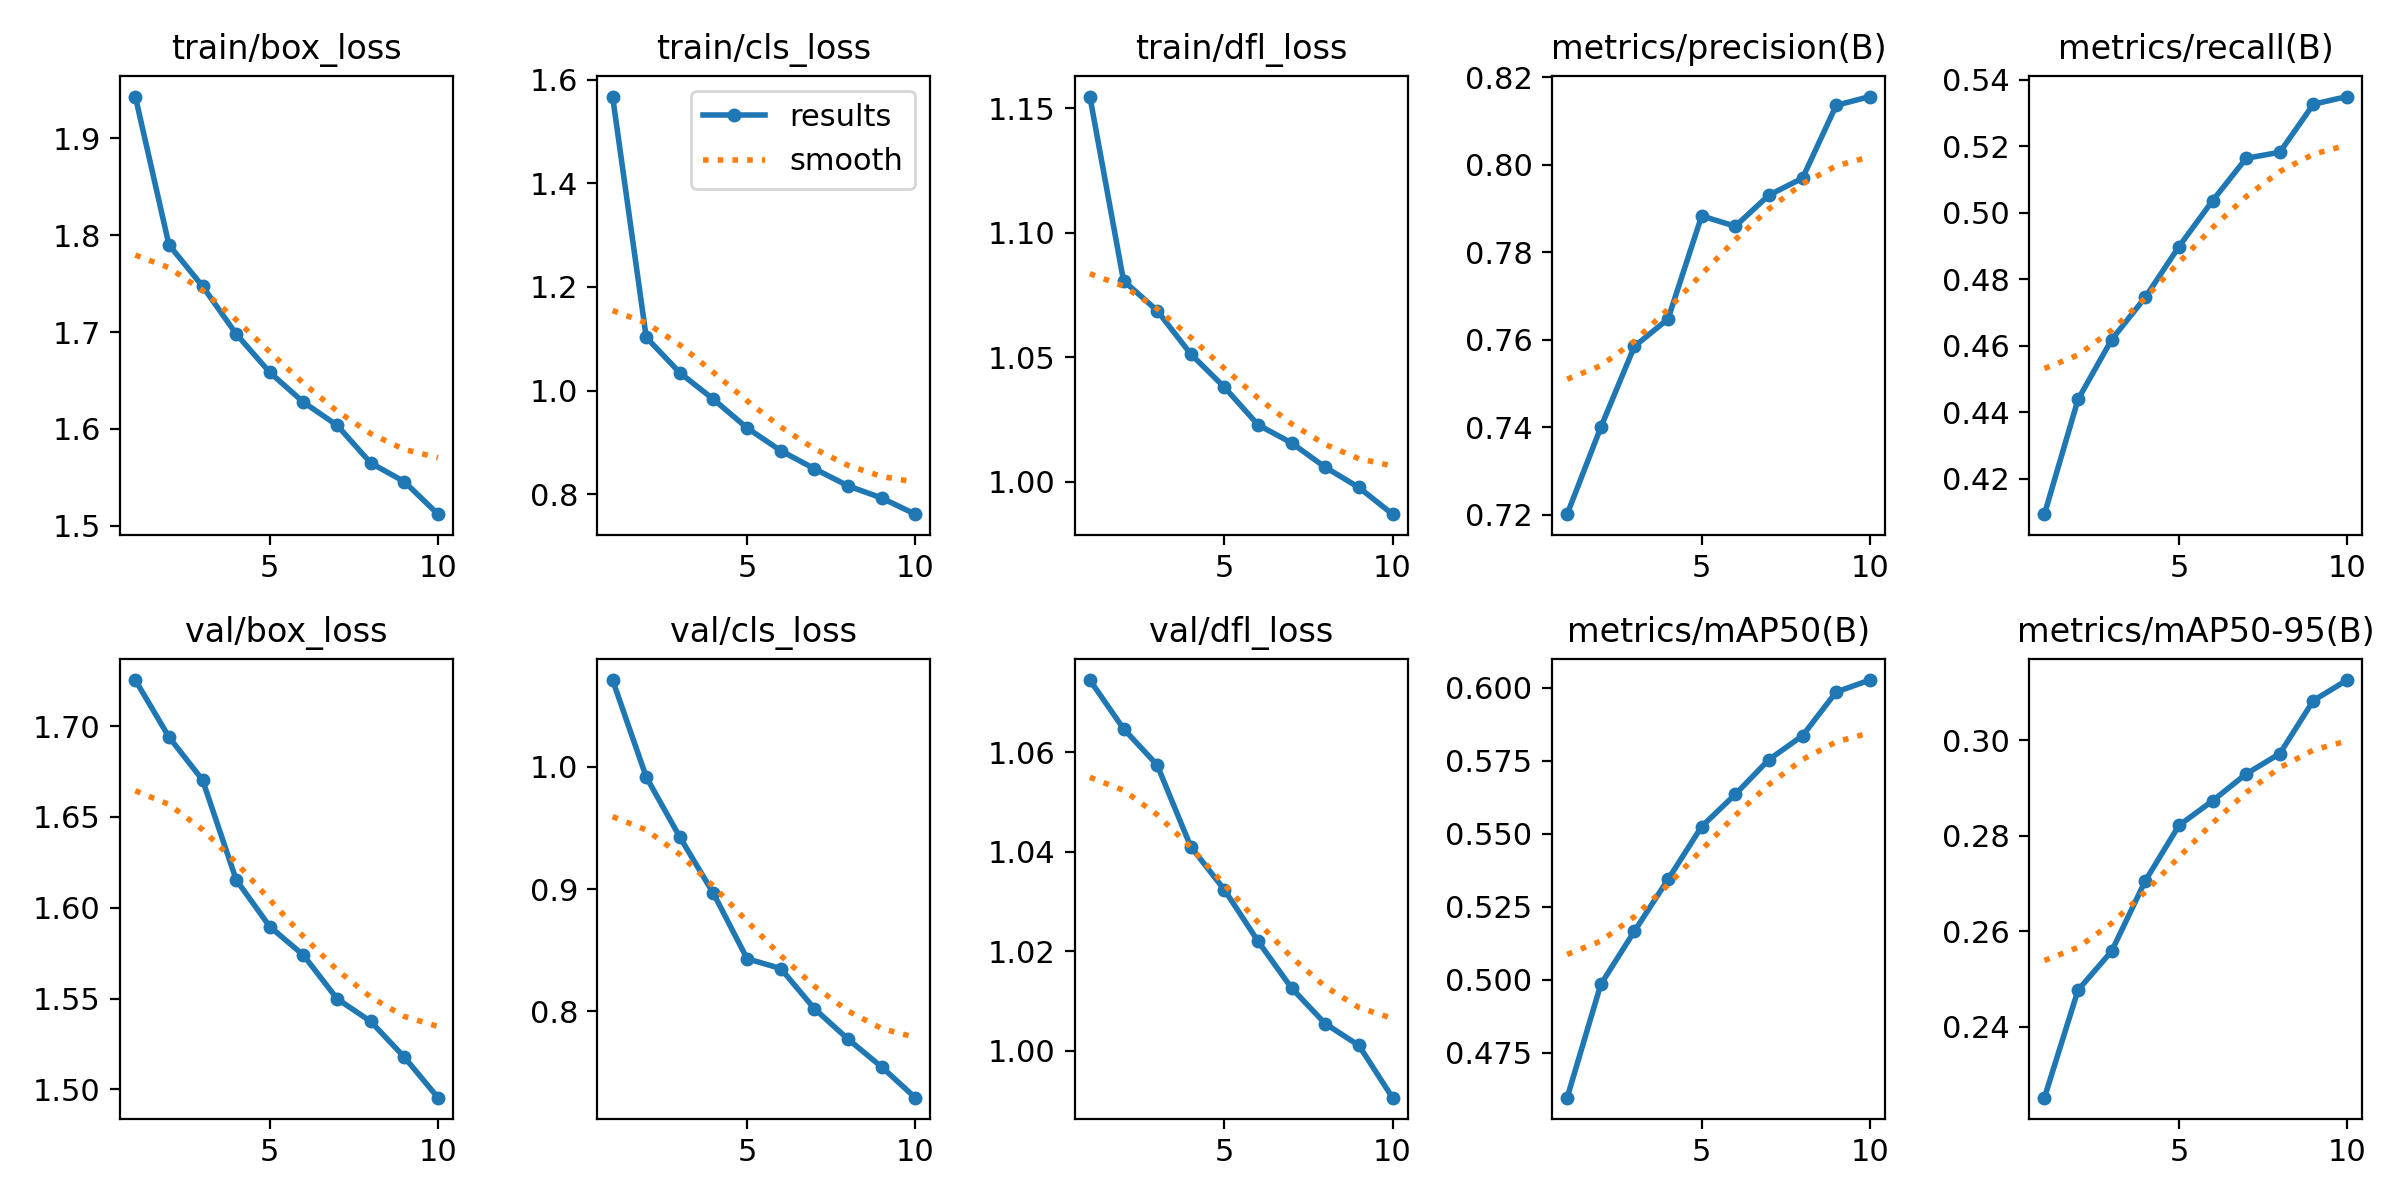
\includegraphics[width=\textwidth]{loss_map.png}
    \caption{روند کاهش توابع هزینه (\lr{Loss}) و افزایش دقت (\lr{mAP}) در داده‌های آموزش و اعتبارسنجی}
    \label{fig:loss_map}
\end{figure}

با بررسی شکل \ref{fig:loss_map}، نتایج زیر به دست می‌آید:
\begin{itemize}
    \item \textbf{عدم بیش‌برازش (\lr{Overfitting}):} نمودارهای ردیف پایین (مربوط به داده‌های \lr{Validation}) دقیقاً مشابه با نمودارهای آموزش (\lr{Train}) دارای روند نزولی پیوسته هستند. عدم افزایشِ مجددِ خطای ولیدیشن نشان می‌دهد که مدل در این ۱۰ دور به حفظ کردن داده‌ها نپرداخته و قدرت تعمیم (\lr{Generalization}) خود را حفظ کرده است.
    \item \textbf{دقت تشخیصِ کادر (\lr{box\_loss} و \lr{dfl\_loss}):} کاهش پیوسته‌ی خطای \lr{Distribution Focal Loss} (DFL) نشان می‌دهد که شبکه به مرور زمان توانسته است لبه‌های کادر محدودکننده (\lr{Bounding Box}) را با اطمینان بیشتری به لبه‌های واقعی چهره نزدیک کند.
    \item \textbf{معیار دقت میانگین (\lr{mAP50}):} رسیدن به دقت بالای ۶۰ درصد (۰.۶۰۳) تنها در ۱۰ دور آموزش برای پایگاه داده‌ی چالش‌برانگیزی مثل \lr{WIDER FACE} که حاوی چهره‌های بسیار ریز و تاریک است، عملکرد فوق‌العاده‌ی معماری \lr{YOLOv8} در یادگیری ویژگی‌ها را اثبات می‌کند.
\end{itemize}

\subsection{ارزیابی کیفی پیش‌بینی‌ها روی تصاویر جدید}

برای ارزیابی نهایی، مدل بر روی سه تصویر تصادفی از مجموعه‌ی اعتبارسنجی که در طول آموزش ندیده بود، اعمال شد. 

\begin{figure}[h!]
    \centering
    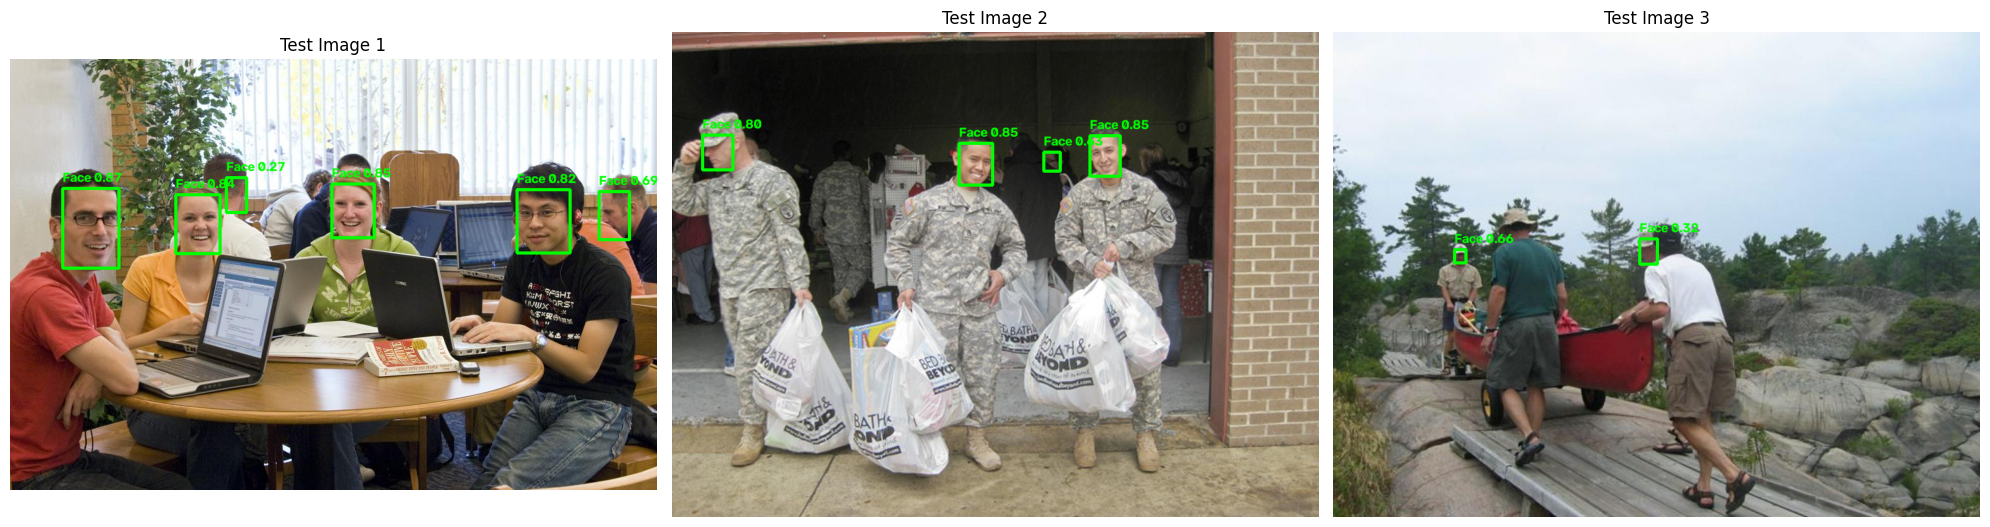
\includegraphics[width=\textwidth]{three_samples.png}
    \caption{عملکرد مدل \lr{Fine-tune} شده بر روی سه نمونه تصویر با شرایط نوری و مقیاس‌های متفاوت}
    \label{fig:three_samples}
\end{figure}

بررسی دقیق تصاویر در شکل \ref{fig:three_samples}، توانمندی‌ها و حساسیت مدل را به خوبی نشان می‌دهد:
\begin{itemize}
    \item \textbf{تصویر اول (سمت چپ):} مدل توانسته چهره‌های اصلی که تمام‌رخ و واضح هستند را با درصد اطمینان بالا (حدود ۰.۸۸) تشخیص دهد. نکته‌ی قابل توجه، تشخیص چهره‌ی یکی از افراد در پس‌زمینه است که سر خود را چرخانده و تنها نیمی از صورت او مشخص است (کادر با اطمینان ۰.۲۷). این موضوع حساسیت بالای مدل به ویژگی‌های جزئیِ چهره را نشان می‌دهد.
    \item \textbf{تصویر دوم (وسط):} با وجود سایه‌ی کلاه‌ها روی صورت و لباس استتار نظامی، مدل به هیچ وجه دچار خطای تشخیص نشده و چهره‌های اصلی را با دقت (۰.۸۰ تا ۰.۸۵) شناسایی کرده است. مدل حتی یک چهره‌ی تاریک در عمق تصویر را نیز موفق شده کادربندی کند.
    \item \textbf{تصویر سوم (سمت راست):} این تصویر چالشی از جنس «تغییر مقیاس» (\lr{Scale}) است. نسبت مساحت چهره‌ها به کل تصویر بسیار ناچیز است، اما شبکه‌ی آموزش‌دیده به لطف رزولوشن ورودی ۶۴۰ پیکسلی، توانسته چهره‌های کوچک را به درستی پیدا کند.
\end{itemize}

\textbf{نتیجه‌گیری بخش:} فرآیند \lr{Fine-tuning} به طور کامل تعصبات (\lr{Biases}) اولیه‌ی مدل خام که بر روی \lr{COCO} آموزش دیده بود (مثل اشتباه گرفتن انسان با میز یا خودرو) را از بین برده و مدل را به یک تشخیص‌دهنده‌ی تخصصی و پایدارِ چهره تبدیل کرده است.